% Orbital rendezvous RL — SHORT interview deck (7 core slides, steers toward strong ground)
% Build: cd interview_deck && tectonic deck_short.tex
\documentclass[aspectratio=169,11pt]{beamer}
\usepackage{amsmath,amssymb,booktabs,tikz,graphicx}
\usetikzlibrary{arrows.meta,positioning,calc}
\graphicspath{{figs/}}

\usetheme{default}
\usecolortheme{seagull}
\definecolor{navy}{HTML}{1F3A5F}
\definecolor{accent}{HTML}{D7301F}
\definecolor{blue2}{HTML}{2C7FB8}
\definecolor{amber}{HTML}{F0A202}
\definecolor{earth}{HTML}{9ECAE1}
\definecolor{grey}{HTML}{666666}
\setbeamercolor{structure}{fg=navy}
\setbeamercolor{title}{fg=navy}
\setbeamercolor{frametitle}{fg=navy,bg=white}
\setbeamercolor{block title}{fg=white,bg=navy}
\setbeamercolor{block body}{bg=navy!6}
\setbeamerfont{frametitle}{series=\bfseries,size=\large}
\setbeamertemplate{navigation symbols}{}
\setbeamertemplate{footline}{\hfill\scriptsize\textcolor{grey}{\insertframenumber}\hspace{3mm}\vspace{2mm}}
\setbeamertemplate{itemize items}[circle]
\newcommand{\key}[1]{\textcolor{accent}{\textbf{#1}}}
\newcommand{\dv}{\ensuremath{\Delta v}}
\newcommand{\nObs}{38}
\newcommand{\nParams}{139{,}281}
\newcommand{\nEnvs}{1024}
\newcommand{\boxR}{30\,km}
\newcommand{\boxV}{50\,m/s}

\title{Learning Orbital Rendezvous}
\subtitle{A reinforcement-learned guidance policy for a chaser spacecraft}
\author{Peter Brown}
\date{October 2026}

\begin{document}

\begin{frame}[plain]
  \titlepage
  \begin{center}\small\textcolor{grey}{One policy, seven rendezvous skills in 3-D with J2, 96--99.5\,\% held-out success on the five wide-box skills.\\ Simulator in C, policy in PyTorch, every number measured on held-out episodes.}\end{center}
  \note{One line: I built a simulator, a guidance policy, and the verification around them, and the policy learned the classical phasing manoeuvre from reward alone. Ten minutes, then questions.}
\end{frame}

% ===================================================================== 1
\begin{frame}{The problem, and the loop that solves it}
\begin{columns}[T]
\begin{column}{0.42\textwidth}
\centering
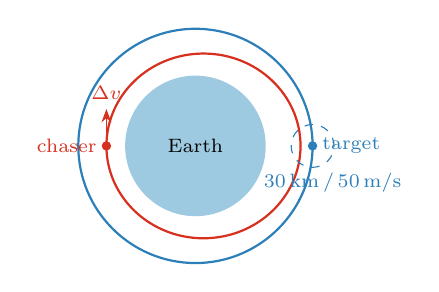
\begin{tikzpicture}[scale=0.85]
  \fill[earth] (0,0) circle (1.05); \node[font=\scriptsize] at (0,0) {Earth};
  \draw[blue2,thick] (0,0) circle (1.75);
  \draw[accent,thick] (0.12,0) ellipse (1.45 and 1.38);
  \fill[accent] (-1.33,0) circle (0.07) node[left,font=\scriptsize,accent] {chaser};
  \fill[blue2] (1.75,0) circle (0.07) node[right,font=\scriptsize,blue2] {target};
  \draw[blue2,dashed] (1.75,0) circle (0.32);
  \node[font=\scriptsize,blue2] at (2.05,-0.55) {\boxR\,/\,\boxV};
  \draw[-{Stealth},accent] (-1.33,0) -- ++(0,0.55) node[above,font=\scriptsize] {\dv};
\end{tikzpicture}
\\[1mm]
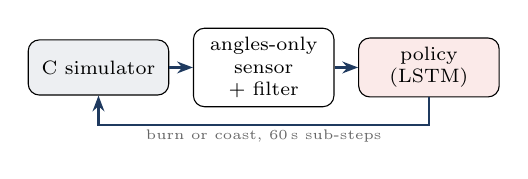
\begin{tikzpicture}[box/.style={draw,rounded corners,minimum height=0.7cm,text width=1.55cm,align=center,font=\scriptsize,fill=white},arr/.style={-{Stealth[length=2mm]},thick,navy}]
  \node[box,fill=navy!8] (sim) {C simulator};
  \node[box,right=0.3cm of sim] (nav) {angles-only sensor + filter};
  \node[box,right=0.3cm of nav,fill=accent!10] (pol) {policy (LSTM)};
  \draw[arr] (sim)--(nav); \draw[arr] (nav)--(pol);
  \draw[arr] (pol.south) |- ++(0,-0.35) -| (sim.south);
  \node[font=\tiny,grey] at ($(sim.south)!0.5!(pol.south)+(0,-0.5)$) {burn or coast, 60\,s sub-steps};
\end{tikzpicture}
\end{column}
\begin{column}{0.58\textwidth}\footnotesize
\textbf{Goal} \; get a chaser inside \boxR\ and \boxV\ of a passive target\\[1mm]
\textbf{Ends when} \; success, or re-entry, escape, empty tank, or the clock runs out\\[1mm]
\textbf{Budget} \; 478\,m/s of \dv\ (15\,\% propellant, Isp 300\,s); about 2.2$\times$ a Hohmann transfer across the band, so no brute force\\[1mm]
\textbf{Start} \; random LEO orbits, any phase gap up to $\pm180^\circ$, independent eccentricity and apse orientation\\[1mm]
\textbf{Sees} \; \nObs\ floats: own elements, fuel, the estimated target, a target-relative block, the clock\\[1mm]
\textbf{Does} \; one of 31 discrete actions: an impulsive burn, or a coast from 1\,min to 24\,h\\[1mm]
{\scriptsize\textcolor{grey}{Target state comes from line-of-sight angles only (batch acquisition, then a recursive filter); the policy flies on that estimate.}}
\end{column}
\end{columns}
\note{The loop is simulator, sensor and filter, policy, action. The sensor line is one sentence: angles only, then a filter; the policy never sees truth in that mode. If pressed on the filter, give the 30-second answer in the briefing and bring it back to the policy result (train on the estimate or lose 46 points).}
\end{frame}

% ===================================================================== 2
\begin{frame}{The physics: analytic two-body, and why a lower orbit catches up}
\begin{columns}[T]
\begin{column}{0.52\textwidth}\small
\textbf{State} \; $(a,e,i,\Omega,\omega,M)$; Cartesian only when needed\\[1mm]
\textbf{Propagate} \; $M \mathrel{+}= n\,\Delta t$ with $n=\sqrt{\mu/a^3}$, then Kepler's equation by Newton
\[ E \leftarrow E - \frac{E - e\sin E - M}{1 - e\cos E},\qquad \tan\tfrac{\theta}{2}=\sqrt{\tfrac{1+e}{1-e}}\tan\tfrac{E}{2} \]
\textbf{Elements $\leftrightarrow$ Cartesian} \; perifocal frame, then $R_3(\Omega)R_1(i)R_3(\omega)$; inverse from $\mathbf h=\mathbf r\times\mathbf v$ and $\mathbf e$ directly\\[1mm]
\textbf{Burns} \; impulsive along $\hat v,\hat r,\hat h$; mass by the rocket equation\\[1mm]
\textbf{J2} \; secular drift of $\Omega$, $\omega$, and the clock\\[1mm]
\textbf{Why analytic} \; exact at any $\Delta t$, so a 24\,h coast is one solve, not 1,440 integrator steps. Roughly half a million env steps per second on one laptop CPU.
\end{column}
\begin{column}{0.48\textwidth}
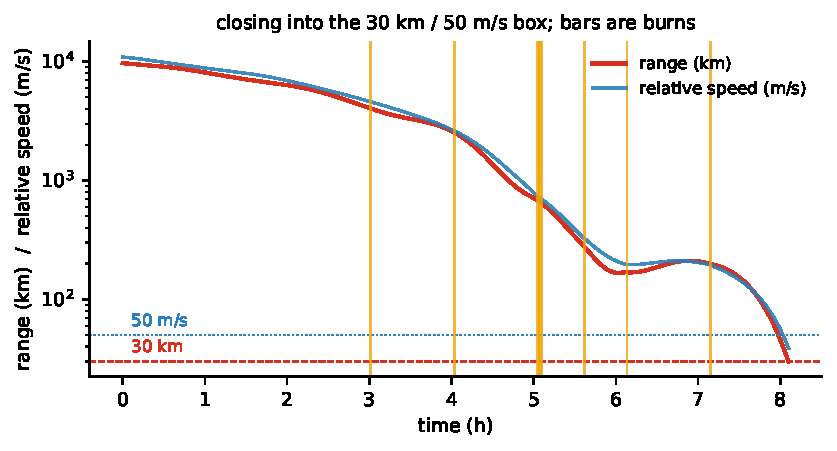
\includegraphics[width=\textwidth]{traj_closing.pdf}
\small\vspace{1mm}
\textbf{Phasing} \; $T=2\pi\sqrt{a^3/\mu}$: 100\,km lower gains about $4^\circ$ per orbit. Drop, wait, raise. The policy rediscovered this; the burns above are it doing so.
\end{column}
\end{columns}
\note{This is home ground. Derivations on the whiteboard: h = r x v is conserved, vis-viva, the conic equation, Kepler. Invite "how did you validate the propagator": energy and angular momentum conserved to float precision; Hohmann 400 to 800 km matches 217 m/s to the metre; an independent f and g oracle agreed to 0.7 m over 600k sub-steps.}
\end{frame}

% ===================================================================== 3
\begin{frame}{Decisions: a small recurrent policy over burns and coasts, trained with PPO}
\begin{columns}[T]
\begin{column}{0.5\textwidth}
\centering
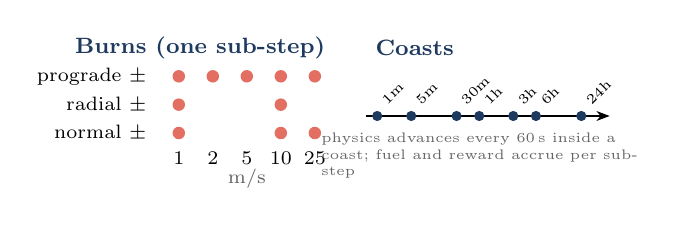
\begin{tikzpicture}[x=0.72cm,y=0.72cm]
  \node[anchor=west,font=\footnotesize\bfseries,navy] at (0,3.0) {Burns (one sub-step)};
  \node[anchor=east,font=\scriptsize] at (1.6,2.5) {prograde $\pm$};
  \foreach \x in {2.0,2.6,3.2,3.8,4.4}{ \fill[accent!70] (\x,2.5) circle (0.11); }
  \node[anchor=east,font=\scriptsize] at (1.6,2.0) {radial $\pm$};
  \foreach \x in {2.0,3.8}{ \fill[accent!70] (\x,2.0) circle (0.11); }
  \node[anchor=east,font=\scriptsize] at (1.6,1.5) {normal $\pm$};
  \foreach \x in {2.0,3.8,4.4}{ \fill[accent!70] (\x,1.5) circle (0.11); }
  \foreach \x/\m in {2.0/1, 2.6/2, 3.2/5, 3.8/10, 4.4/25}{ \node[font=\scriptsize] at (\x,1.05) {\m}; }
  \node[font=\scriptsize,grey] at (3.2,0.7) {m/s};
  \node[anchor=west,font=\footnotesize\bfseries,navy] at (5.3,3.0) {Coasts};
  \draw[-{Stealth}] (5.3,1.8) -- (9.6,1.8);
  \foreach \x/\lab in {5.5/1m, 6.1/5m, 6.9/30m, 7.3/1h, 7.9/3h, 8.3/6h, 9.1/24h}{ \fill[navy] (\x,1.8) circle (0.09); \node[font=\tiny,rotate=45,anchor=west] at (\x,1.92) {\lab}; }
  \node[font=\tiny,grey,text width=4.3cm] at (7.5,1.1) {physics advances every 60\,s inside a coast; fuel and reward accrue per sub-step};
\end{tikzpicture}
\vspace{3mm}
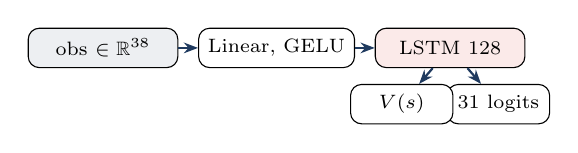
\begin{tikzpicture}[nb/.style={draw,rounded corners,minimum width=1.9cm,minimum height=0.5cm,font=\scriptsize,fill=white},arr/.style={-{Stealth[length=1.8mm]},thick,navy}]
  \node[nb,fill=navy!8] (o) {obs $\in\mathbb R^{\nObs}$};
  \node[nb,right=0.25cm of o] (e) {Linear, GELU};
  \node[nb,right=0.25cm of e,fill=accent!10] (l) {LSTM 128};
  \node[nb,below right=0.2cm and -1.0cm of l,minimum width=1.3cm] (a) {31 logits};
  \node[nb,below left=0.2cm and -1.0cm of l,minimum width=1.3cm] (v) {$V(s)$};
  \draw[arr] (o)--(e); \draw[arr] (e)--(l); \draw[arr] (l)--(a); \draw[arr] (l)--(v);
\end{tikzpicture}
\end{column}
\begin{column}{0.5\textwidth}\footnotesize
\textbf{Semi-Markov} \; one decision spans 60\,s to 24\,h; the headline policy takes \key{24 decisions} per episode. Without coasts the credit horizon is thousands of steps and nothing learns.\\[1.2mm]
\textbf{Why an LSTM} \; what a burn did, and whether the estimate is settling, live in the history, not the current frame. \nParams\ parameters.\\[1.2mm]
\textbf{PPO} \; \nEnvs\ parallel envs, $\gamma=0.995$, clipped surrogate $\pm0.2$, GAE, entropy bonus; 50\,M steps per rung, about 2\,h each on a laptop.\\[1.2mm]
\textbf{Reward} \; $+1$ arrive, $-1$ fail, plus a potential-difference hint per decision on the mean-longitude gap and element match, clamped to $[-1,1]$.\\[1.2mm]
\textbf{Curriculum} \; warm-start one variable per rung: circular at the full gap $\to$ eccentric $\to$ wide envelope $\to$ 3-D $\to$ estimate in the loop $\to$ seven-skill mixture.
\end{column}
\end{columns}
\note{Strong ground: PPO steps (rollout 1024 envs, advantages by GAE, clipped ratio, few epochs), why the clamp (bounds the gradient from rare terminal events), why potential shaping does not change the optimum (telescoping with gamma_shape = 1). If asked about continuous actions: tried Box(2), entropy collapsed; discrete grades are simpler for PPO.}
\end{frame}

% ===================================================================== 4
\begin{frame}{What it learned, 2-D: every held-out episode rendezvous, on every training seed}
\centering
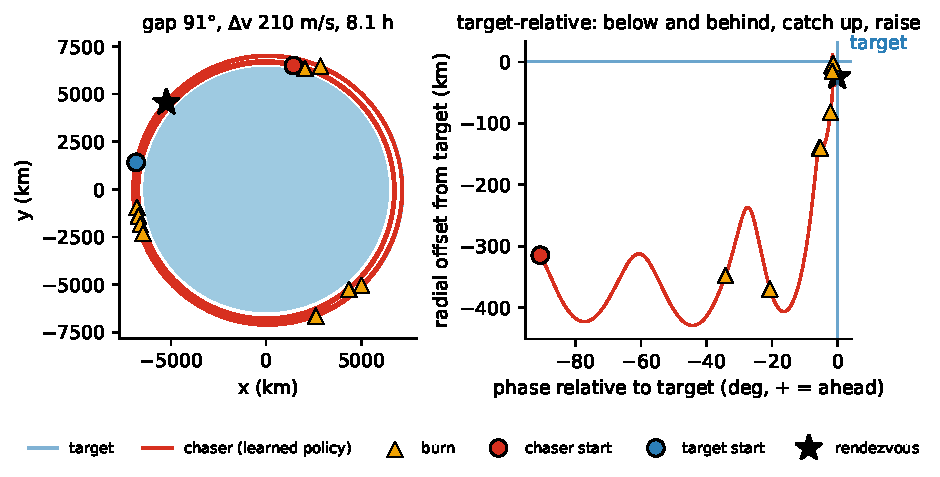
\includegraphics[width=0.62\textwidth]{traj_rendezvous.pdf}
\begin{columns}[T]
\begin{column}{0.6\textwidth}\footnotesize
\begin{itemize}
  \item \key{200/200} held-out episodes for \key{5/5 training seeds}, including the seed that flat-lined at 0\,\% before the dynamics fix.
  \item Re-run for this deck on a fresh evaluation seed: 200/200.
  \item Wide envelope (300--8,000\,km, $e\le0.30$): 4 seeds, 800/800.
\end{itemize}
\end{column}
\begin{column}{0.38\textwidth}\scriptsize\textcolor{grey}{A $91^\circ$ gap closed in 8.1\,h with 210\,m/s: below and behind, let the lower orbit catch up, then raise in steps. Median fuel is 1.18$\times$ a two-impulse optimum on the same clock (appendix).}
\end{column}
\end{columns}
\note{Point at the burn triangles: early retrograde to drop, then prograde to raise. The right panel is the whole strategy. If asked about fuel: 1.18x the time-matched two-impulse optimum; the policy trades about 20 percent fuel for faster closure; the comparator is in the appendix if they want it.}
\end{frame}

% ===================================================================== 5
\begin{frame}{One policy, seven rendezvous skills, 3-D with J2}
\begin{columns}[T]
\begin{column}{0.5\textwidth}
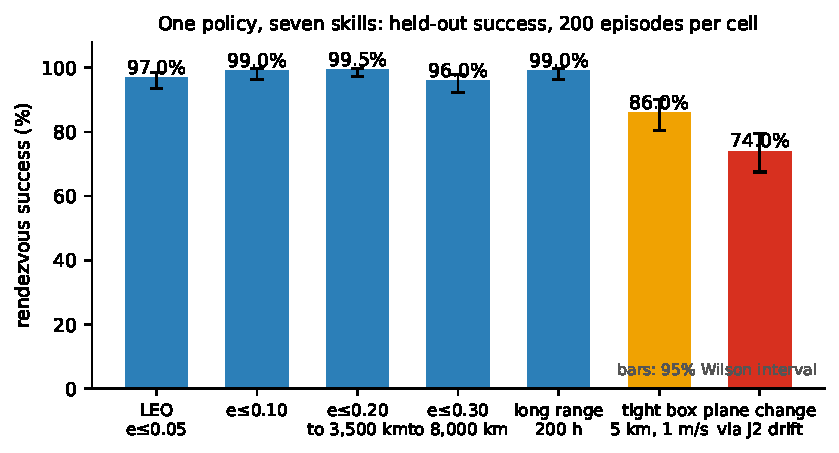
\includegraphics[width=\textwidth]{generalist_cells.pdf}
\end{column}
\begin{column}{0.5\textwidth}
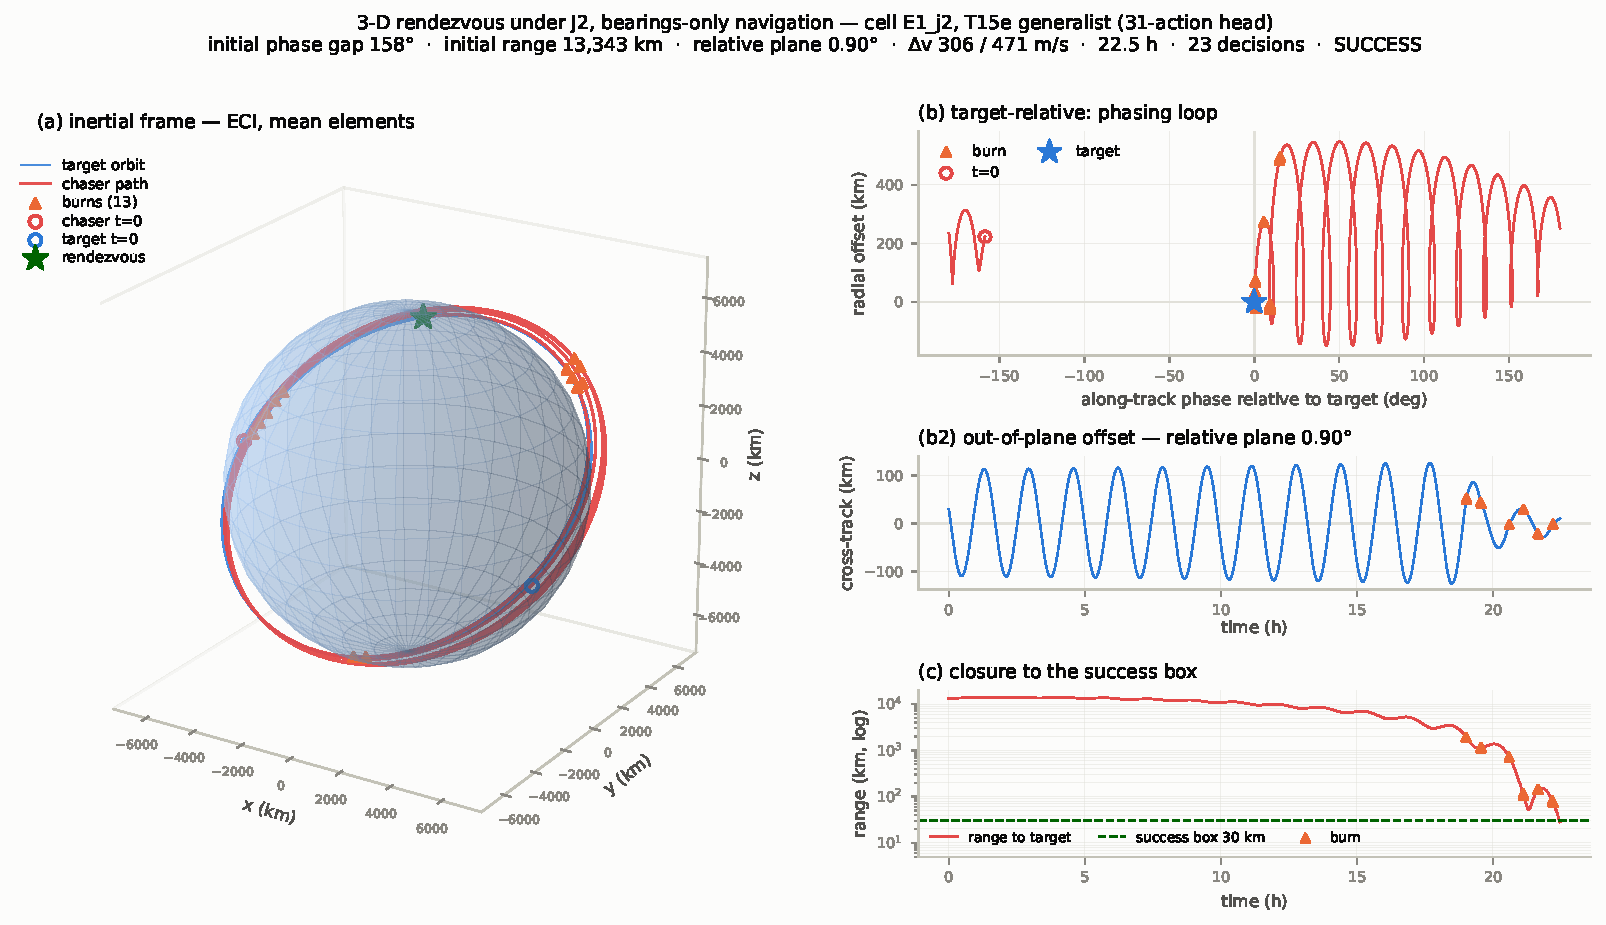
\includegraphics[width=\textwidth]{traj3d_rendezvous.pdf}
\end{column}
\end{columns}
\vspace{-1mm}
{\scriptsize\textcolor{grey}{Left: held-out success per skill, 200 episodes each, bearings-only navigation; six of the seven skills reproduce at a second training seed; tight box reaches 92.5\,\% at its training fuel floor. Right: one held-out episode, a $158^\circ$ gap and a $0.9^\circ$ plane difference closed in 22.5\,h with 306\,m/s and 23 decisions. The seventh skill waits for J2 nodal precession to close a plane gap that burning could not afford.}}
\note{Centrepiece. Five skills at 96 to 99.5, tight box 86 (92.5 at training floor), plane change 74. Talk the physics of the seventh skill: dOmega/dt depends on altitude and inclination, so parking at a different altitude makes the planes drift together; a 3 degree change by burning would exceed the tank. Single-skill specialists score 6 to 42 percent off their home cell, which is why one policy was worth building.}
\end{frame}

% ===================================================================== 6
\begin{frame}{How it got there: interference measured, then fixed}
\begin{columns}[T]
\begin{column}{0.5\textwidth}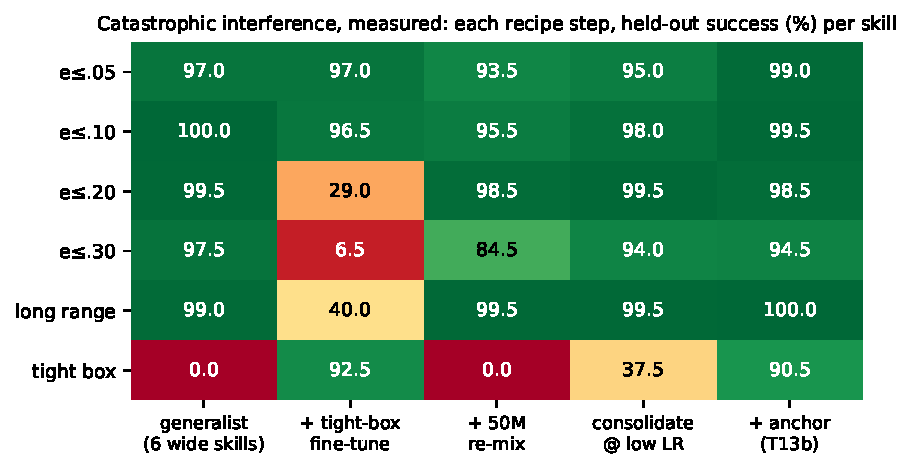
\includegraphics[width=\textwidth]{seesaw.pdf}\end{column}
\begin{column}{0.5\textwidth}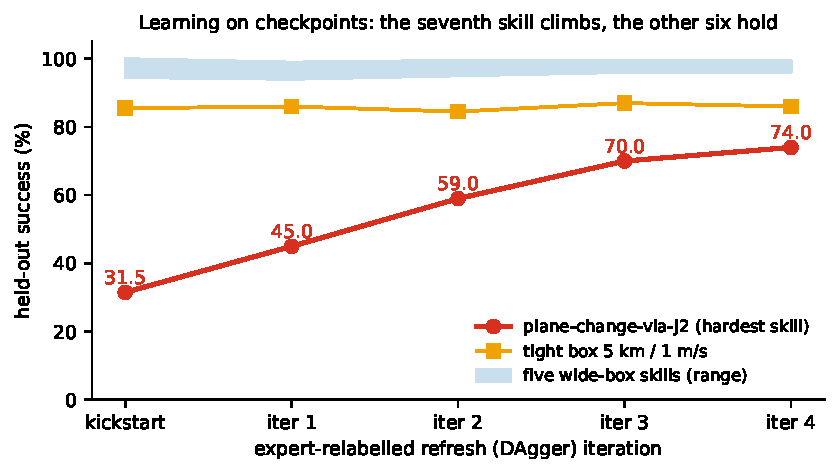
\includegraphics[width=\textwidth]{dagger_curve.pdf}\end{column}
\end{columns}
\small
\begin{itemize}
  \item Fine-tuning for the tight box destroyed three other skills; re-mixing restored them and lost the tight box. Low-learning-rate consolidation with an \key{anchor} (replay of the specialist's own trajectories) held all six.
  \item The seventh skill never bootstrapped from reward. It came from four rounds of \key{expert-relabelled refresh} against a scripted expert, with a stopping rule fixed in advance; reproduced at a second seed.
\end{itemize}
\note{This is the ML story and the honest answer to "where is your training curve": every point here is a 200-episode held-out eval of a checkpoint. Catastrophic interference, replay anchors, DAgger: all things you can explain from first principles.}
\end{frame}

% ===================================================================== 7
\begin{frame}{What I caught, what is open, what is next}
\begin{columns}[T]
\begin{column}{0.5\textwidth}\footnotesize
\textbf{Caught}
\begin{itemize}
  \item A swapped half-angle factor in the true-to-mean anomaly conversion let every burn teleport phase (median $25^\circ$ per episode). The old headline fell from 97.5\,\% to 13\,\% once fixed; everything here is post-fix.
  \item A reward leak that made coast-only policies look capable at high altitude (null test: a zero policy reproduced it).
  \item A numbered ledger of metric-versus-implementation bugs, each with a before/after number.
\end{itemize}
\textbf{Also built} \; a two-impulse Lambert comparator for the fuel audit; a bearings-only navigation stack; an allocation-free C port of the policy, action-for-action identical to PyTorch.
\end{column}
\begin{column}{0.5\textwidth}\footnotesize
\textbf{Open}
\begin{itemize}
  \item The seventh skill's final refinement chain is one training seed; six skills reproduce at a second seed.
  \item Fuel is 1.18$\times$ the two-impulse optimum, not 1.0; the burn grid is coarse.
  \item Chaser navigation assumed perfect; no eclipses or sensor bias; arrival certified, not station-keeping.
\end{itemize}
\textbf{Next}
\begin{itemize}
  \item A matched MPC comparator; a maneuvering target.
  \item Finer burn grades; multi-seed the generalist.
\end{itemize}
\end{column}
\end{columns}
\note{Close on the bug. Posture: I would rather show you the bug I found than a number I cannot defend. The "also built" line names the three weak areas once, briefly, on your terms. Then questions.}
\end{frame}

% ===================================================================== appendix
\appendix
\begin{frame}[plain]\centering{\Large\textcolor{navy}{\textbf{Appendix}}}\\[2mm]\small observation vector \;$\cdot$\; J2 and phasing \;$\cdot$\; the seven cells \;$\cdot$\; the dynamics bug \;$\cdot$\; fuel audit \;$\cdot$\; navigation in one picture \;$\cdot$\; C port \;$\cdot$\; if asked\end{frame}

\begin{frame}{A1 \; Observation vector (\nObs\ floats, roughly in $[-1,1]$)}
\tiny
\begin{tabular}{@{}lll@{}}
\toprule
slots & value & why\\
\midrule
0--1 & chaser altitude / scale, $e$ & size and shape\\
2--3 & $\sin\theta,\cos\theta$ & position on orbit, no wrap\\
4--5 & $v_r/v_{circ},\ v_t/v_{circ}$ & radial and tangential speed\\
6 & fuel fraction & budget remaining\\
7--8 & target altitude, $e$ (estimated) & target size and shape\\
9--12 & $\sin,\cos\,\omega$ for both & apse orientations\\
13--14 & $\sin,\cos\,\Delta\lambda$ (mean-longitude gap) & the phase gap\\
15 & (cap $-$ step)/cap & episode clock\\
16 & $\cos(\omega_s-\omega_t)$ & apsidal alignment\\
17--20 & nearest body: distance, bearing, closing rate, keep-out & Earth\\
21--25 & relative-inclination vector; $\Delta\mathbf e\cdot\hat h_t$; cross-track offset and rate & 3-D block\\
26--28 & $\dv_{plane},\ \dv_{remaining}$, feasibility margin & fuel ledger\\
29--30 & $\cos i_s,\ \cos i_t$ & J2\\
33--36 & LVLH radial / along-track offset; relative velocity, rotating-frame corrected & relative state\\
37 & target mean motion & \\
\bottomrule
\end{tabular}
\\[1mm]\textcolor{grey}{Target quantities are the filter's estimate in bearings-only mode. The policy is not given the covariance (tested: a $\sigma$ channel added nothing).}
\end{frame}

\begin{frame}{A2 \; Plane change by burning versus by J2}
\small
\textbf{By burning} \; $\dv = 2v\sin(\Delta i/2)$. At 7.5\,km/s a $3^\circ$ change costs about 390\,m/s, most of a 478\,m/s tank.\\[2mm]
\textbf{By J2} \; Earth's equatorial bulge makes the orbit's node line drift around the pole at
\[ \dot\Omega = -\tfrac32\, J_2\, n \left(\frac{R_E}{p}\right)^{2} \cos i, \qquad p = a(1-e^2). \]
The rate depends on altitude and inclination, so two orbits at different altitudes drift apart in $\Omega$ at a controllable relative rate. Dip low, coast a day at a time, let the node drift close the plane gap, then raise. In the specialist about half of the plane alignment was bought this way; the rest with normal burns near the relative node.\\[2mm]
\textbf{Phasing} \; $T = 2\pi\sqrt{a^3/\mu}$; a chaser 100\,km below a LEO target gains about $4^\circ$ of phase per orbit, so "drop, wait $N$ orbits, raise" is the textbook catch-up and it is what the policy does.
\end{frame}

\begin{frame}{A3 \; The seven cells}
\scriptsize
\begin{tabular}{@{}lllllr@{}}
\toprule
cell & altitude band (km) & $e_{max}$ & box & clock (sub-steps) & success\\
\midrule
E0\_j2 & 300--800 & 0.05 & \boxR\,/\,\boxV & 3,000 & 97.0\,\%\\
E1\_j2 & 300--1,500 & 0.10 & \boxR\,/\,\boxV & 3,000 & 99.0\,\%\\
E2\_j2 & 300--3,500 & 0.20 & \boxR\,/\,\boxV & 4,500 & 99.5\,\%\\
E3\_j2 & 300--8,000 & 0.30 & \boxR\,/\,\boxV & 6,000 & 96.0\,\%\\
LONGRANGE & 300--3,500 & 0.12 & \boxR\,/\,\boxV & 12,000 & 99.0\,\%\\
TIGHT\_5k1 & 300--800 & 0.05 & 5\,km\,/\,1\,m/s & 3,000 & 86.0\,\%$^\dagger$\\
W1\_driftwait & 300--800 & 0.05 & \boxR\,/\,\boxV & 22,000 & 74.0\,\%\\
\bottomrule
\end{tabular}
\\[2mm]
$^\dagger$92.5\,\% at the training fuel floor. All cells: 3-D, J2 on, targets inclined $30$--$60^\circ$, relative plane up to $0.75$--$1^\circ$ ($2$--$5^\circ$ for W1), bearings-only navigation, Discrete(31) head, fuel budget sampled per episode (353--656\,m/s). Held-out seed 123, 200 episodes per cell, greedy actions, LSTM state zeroed per episode.
\end{frame}

\begin{frame}{A4 \; The dynamics bug}
\small
\begin{columns}[T]
\begin{column}{0.5\textwidth}
\textbf{What} \; the true-anomaly $\to$ mean-anomaly conversion, called only after a burn, had its $\sqrt{1\pm e}$ factors swapped. Each burn off an apse silently moved the chaser along-track (up to 700\,km at $e=0.05$); a median $25^\circ$ of free phasing per episode. Burns at apsides were unaffected, so every unit test passed.\\[2mm]
\textbf{Found} \; twice on one day: by formula inspection while porting the dynamics into the navigation code, and by the fuel audit, where 15\,\% of episodes beat half the two-impulse optimum on the same clock.\\[2mm]
\textbf{Cost} \; the then-canonical checkpoint went from 97.5\,\% to 13\,\% under corrected dynamics. All pre-fix checkpoints and numbers were retired.
\end{column}
\begin{column}{0.5\textwidth}
\textbf{Recovery} (each piece ablated)
\begin{itemize}
  \item potential shaping on the \emph{mean-longitude} gap with $\gamma_{shape}=1$
  \item physical-gap initialisation and a fixed phase observation
  \item an episode-clock observation; cap reward 0, not $-10$
  \item scripted GNC expert as a reference: 99.2\,\%
\end{itemize}
\textbf{Lesson} \; the comparator caught what the success metric could not. Audits against physics belong in the training loop.
\end{column}
\end{columns}
\end{frame}

\begin{frame}{A5 \; Fuel audit against a two-impulse optimum}
\begin{columns}[T]
\begin{column}{0.56\textwidth}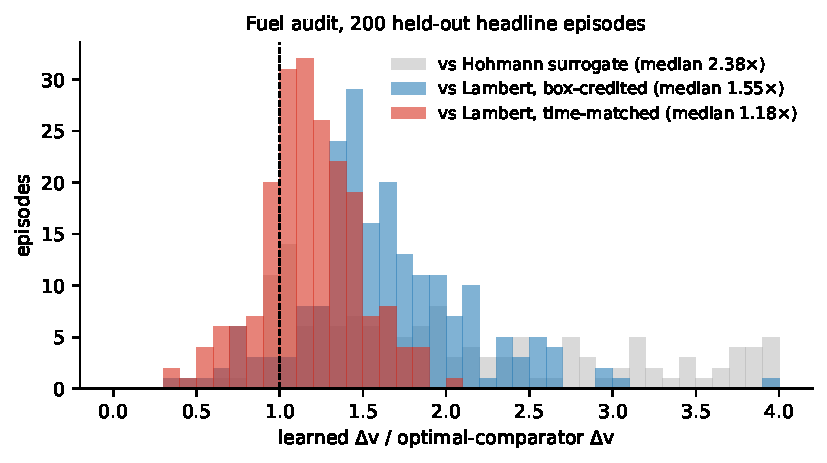
\includegraphics[width=\textwidth]{dv_ratio.pdf}\end{column}
\begin{column}{0.44\textwidth}\footnotesize
For each episode an offline solver finds the cheapest two-burn transfer from the chaser's start to the target's position at arrival, searching over how long to wait before the first burn and how long to fly, on the same clock the policy used.\\[1.5mm]
Median learned \dv\ is \key{1.18$\times$} that optimum (time-matched); 1.55$\times$ when the optimum is credited the box's 50\,m/s velocity tolerance.\\[1.5mm]
{\scriptsize\textcolor{grey}{200 held-out episodes. Ratios below 1 happen because arrival is credited inside a box, not at an exact state, and a two-burn plan is not the unconstrained optimum.}}
\end{column}
\end{columns}
\end{frame}

\begin{frame}{A6 \; Navigation in one picture: blind, acquire, converge}
\centering
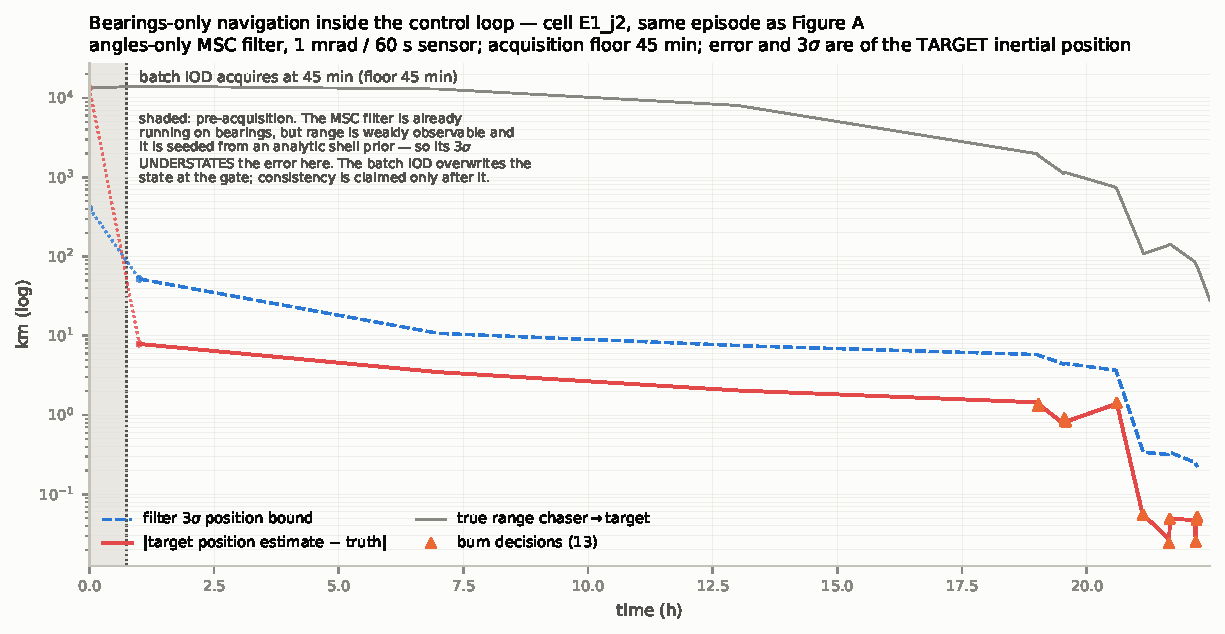
\includegraphics[width=0.72\textwidth]{nav3d_estimate.pdf}
\begin{columns}[T]
\begin{column}{0.5\textwidth}\scriptsize
The chaser measures only the direction to the target, not the distance. One direction tells you nothing about range; a sequence of directions while both orbits curve does. A batch solver tries many ranges along the first line of sight, propagates each, and keeps the one whose predicted directions match what was seen. That hands a full state to a recursive filter that keeps refining it.
\end{column}
\begin{column}{0.5\textwidth}\scriptsize
Policy result: trained on truth and handed the estimate, \key{51\,\%}; trained with the filter in the loop, \key{97\,\%} (2-D tight box) and \key{46$\to$98\,\%} across three seeds in 3-D. It learned to wait for acquisition and burn nothing while blind (median \dv\ before acquisition 75$\to$0\,m/s).
\end{column}
\end{columns}
\end{frame}

\begin{frame}{A7 \; C port of the policy}
\begin{columns}[T]
\begin{column}{0.5\textwidth}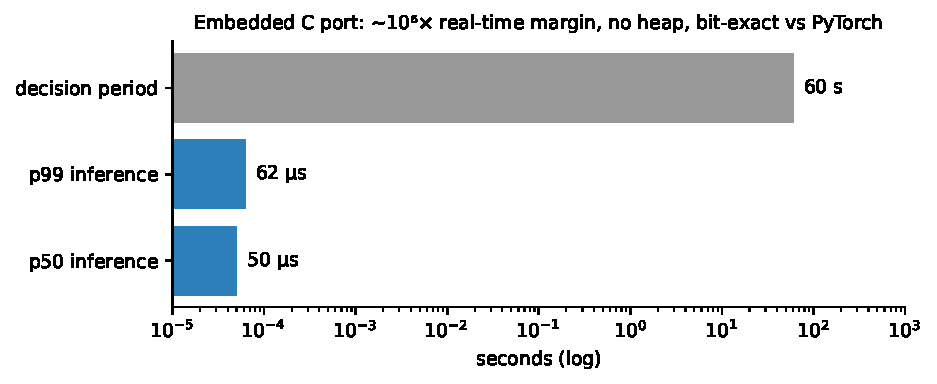
\includegraphics[width=0.95\textwidth]{cport_timing.pdf}\\[2mm]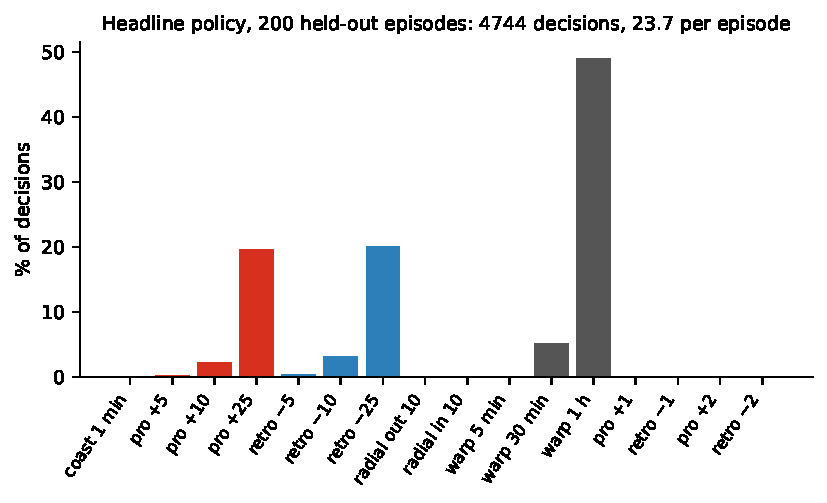
\includegraphics[width=0.95\textwidth]{action_hist.pdf}\end{column}
\begin{column}{0.5\textwidth}\footnotesize
\begin{itemize}
  \item The trained weights exported to a C header; forward pass written by hand: linear, GELU, LSTM cell, two linear heads.
  \item No heap, no globals; the caller owns the 1\,kB of recurrent state; fixed work per call.
  \item Checked against PyTorch: identical action on 7,048 recorded observations and an identical action stream over 200 closed-loop episodes.
  \item Median 50\,$\mu$s per decision on a laptop against a 60\,s decision period (a benchmark, not a worst-case timing).
  \item Bottom: what the headline policy actually does, per decision: warps and prograde/retrograde 25\,m/s dominate.
\end{itemize}
\end{column}
\end{columns}
\end{frame}

\begin{frame}{A8 \; FAQ}
\scriptsize
\begin{description}
  \item[Why RL, when Lambert exists?] Lambert needs perfect state and gives an open-loop two-burn plan; the policy is closed-loop on an estimate, respects a budget, and one network covers seven regimes. Lambert is the grader, not the competitor.
  \item[Why discrete actions?] PPO is stable with them; a continuous head collapsed early on. The grid costs fuel (1.14--1.18$\times$ across two evaluation sets); finer grades are the obvious next step.
  \item[Why not MPC?] It is the right production baseline and the comparison I would run next, with the same filter in the loop.
  \item[Is 200 episodes enough?] At 97\,\% the 95\,\% Wilson interval is about $\pm2.5$\,pp; for 0/200 failures the lower bound is 98.2\,\%. I report intervals, not "100\,\%".
  \item[Single seed?] The six-skill policy reproduced at a second training seed (tight box 92.5\,\%, wide cells 93.5--100\,\%). The seventh skill's four-step refinement was run once by design; its first two steps reproduced at a second seed with matching gains. The 2-D headline (5), wide envelope (4), 3-D nav and J2 rungs (3) are multi-seed.
  \item[Why coast 24\,h?] J2 nodal precession closes a plane gap for free; burning it would exceed the tank. The policy learned to wait.
  \item[How does the filter work?] Angles only, so range comes from how the bearing changes while the orbits curve; a batch solver picks the range that explains the first hour of bearings, then a recursive filter refines it. The finding I own is on the policy side: train on the estimate or lose 46 points.
  \item[What would you do differently?] Audit against physics from day one; log learning curves on every run; design the observation with the filter in mind from the start.
\end{description}
\end{frame}

\end{document}
